%iffalse
\documentclass[journal]{IEEEtran}
\usepackage[a5paper, margin=10mm]{geometry}
%\usepackage{lmodern} % Ensure lmodern is loaded for pdflatex
\usepackage{tfrupee} % Include tfrupee package


\setlength{\headheight}{1cm} % Set the height of the header box
\setlength{\headsep}{0mm}     % Set the distance between the header box and the top of the text


%\usepackage[a5paper, top=10mm, bottom=10mm, left=10mm, right=10mm]{geometry}

%
\setlength{\intextsep}{10pt} % Space between text and floats

\makeindex


\usepackage{cite}
\usepackage{amsmath,amssymb,amsfonts,amsthm}
\usepackage{algorithmic}
\usepackage{graphicx}
\usepackage{textcomp}
\usepackage{xcolor}
\usepackage{txfonts}
\usepackage{listings}
\usepackage{enumitem}
\usepackage{mathtools}
\usepackage{gensymb}
\usepackage{comment}
\usepackage[breaklinks=true]{hyperref}
\usepackage{tkz-euclide} 
\usepackage{listings}
\usepackage{multicol}
\usepackage{xparse}
\usepackage{gvv}
%\def\inputGnumericTable{}                                 
\usepackage[latin1]{inputenc}                                
\usepackage{color}                                            
\usepackage{array}                                            
\usepackage{longtable}                                       
\usepackage{calc}                                             
\usepackage{multirow}                                         
\usepackage{hhline}                                           
\usepackage{ifthen}  
\usepackage{esint}
\usepackage{lscape}
\usepackage{tabularx}
\usepackage{array}
\usepackage{float}
\usepackage[justification=centering]{caption}


\newtheorem{theorem}{Theorem}[section]
\newtheorem{problem}{Problem}
\newtheorem{proposition}{Proposition}[section]
\newtheorem{lemma}{Lemma}[section]
\newtheorem{corollary}[theorem]{Corollary}
\newtheorem{example}{Example}[section]
\newtheorem{definition}[problem]{Definition}
\newcommand{\BEQA}{\begin{eqnarray}}
\newcommand{\EEQA}{\end{eqnarray}}

\theoremstyle{remark}


\begin{document}

\bibliographystyle{IEEEtran}
\onecolumn

\title{Naval Architecture and Marine Engineering}
\author{EE25BTECH11026-Harsha}
\maketitle

\renewcommand{\thefigure}{\theenumi}
\renewcommand{\thetable}{\theenumi}
\setcounter{secnumdepth}{0}
\subsection{\underline{\textbf{General Aptitude (G.A)}}}
\subsubsection{\underline{Q.1 \text{-} Q.5 Carry ONE mark Each}}
\setlength{\parskip}{1em}

\begin{enumerate}[itemsep=1em]
\item "You are delaying the completion of the task. Send \underline{\hspace{2cm}} contributions at the earliest".
\begin{multicols}{4}
\begin{enumerate}
      \item you are
      \item your
      \item you're
      \item yore
\end{enumerate}
\end{multicols}
\end{enumerate}

\begin{enumerate}[itemsep=1em]
\setcounter{enumi}{1}
\item References : \underline{\hspace{1cm}} :: Guidelines : Implement (By word meaning) 

\begin{multicols}{4}
\begin{enumerate}
       \item Sight
       \item Site
       \item Cite
       \item Plagiarise
\end{enumerate}
\end{multicols}
\end{enumerate}

\begin{enumerate}[itemsep=1em]
\setcounter{enumi}{2}
\item In the given figure, $PQRS$ is a parallelogram with PS=$7$ cm, PT=$4$ cm and PV=$5$ cm. What is the length of RS in cm? (The diagram is representative.)  
\begin{figure}[H]
    \centering
    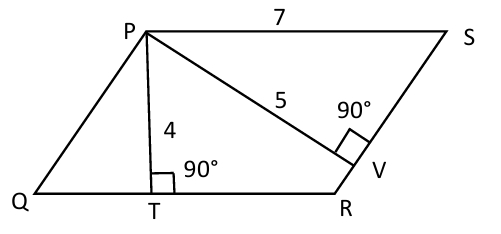
\includegraphics[width=0.4\columnwidth]{figs/fig-1.jpeg}
    \caption*{Fig-1:Parelleogram PQRS}
    \label{fig-1}
\end{figure}
\begin{multicols}{4}
\begin{enumerate}
     \item $\frac{20}{7}$
     \item $\frac{28}{5}$
     \item $\frac{9}{2}$
     \item $\frac{35}{4}$
\end{enumerate}
\end{multicols}
\end{enumerate}
\newpage
\vspace*{0.25cm}
\begin{enumerate}[itemsep=1em]
\setcounter{enumi}{3}
\item In $2022$, June Huh was awarded the Fields medal, which is the highest prize in Mathematics.When he was younger, he was also a poet. He did not win any medals in the International Mathematics Olympiads. He dropped out of college.Based only on the above information, which one of the following statements can be logically inferred with certainty?
\begin{enumerate}[leftmargin=2.5em, labelsep=0.5em, itemsep=0.5em]
    \item Every Fields medalist has won a medal in an International Mathematics Olympiad.
    \item Everyone who has dropped out of college has won the Fields medal. 
    \item All Fields medalists are part-time poets. 
    \item Some Fields medalists have dropped out of college. 
\end{enumerate}
\end{enumerate}

\begin{enumerate}[itemsep=1em]
\setcounter{enumi}{4}
\item A line of symmetry is defined as a line that divides a figure into two parts in a way such that each part is a mirror image of the other part about that line. \\ 
The given figure consists of $16$ unit squares arranged as shown. In addition to the three black squares, what is the minimum number of squares that must be coloured black, such that both PQ and MN form lines of symmetry?                        (The figure is representative) 
\begin{figure}[H]
    \centering
    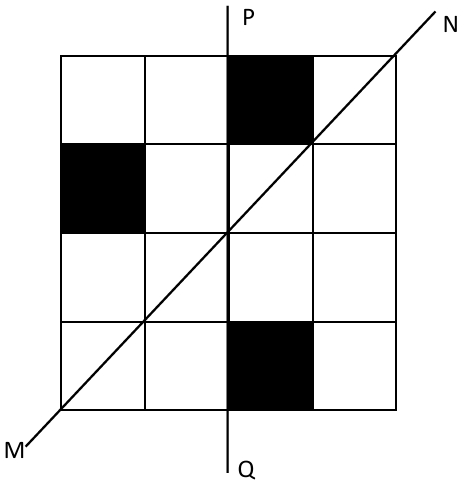
\includegraphics[width=0.4\columnwidth]{figs/fig-2.jpeg}
    \caption*{Fig-2}
    \label{fig-2}
\end{figure}
\begin{multicols}{4}
\begin{enumerate}
      \item $3$
      \item $4$
      \item $5$
      \item $6$
\end{enumerate}
\end{multicols}
\end{enumerate}

\newpage
\vspace*{0.25cm}

\subsubsection{\underline{Q.6 \text{-} Q.10 Carry TWO mark Each}}
\begin{enumerate}[itemsep=1em]
\setcounter{enumi}{5}
\item Human beings are one among many creatures that inhabit an imagined world. In this imagined world, some creatures are cruel. If in this imagined world, it is given that the statement 'Some human beings are not cruel creatures' is FALSE, then which of the following sets of statements be logically inferred with certainty? \\
(i) All human beings are cruel creatures. \\
(ii) Some human beings are cruel creatures. \\
(iii) Some creatures that are cruel are human beings. \\
(iv) No human beings are cruel creatures.\\
\begin{multicols}{4}
\begin{enumerate}
     \item only (i) 
     \item only (iii) and(iv) 
     \item only (i) and (ii) 
     \item (i),(ii) and (iii) 
\end{enumerate}
\end{multicols}
\end{enumerate}

\begin{enumerate}[itemsep=1em]
\setcounter{enumi}{6}
\item To construct a wall, sand and cement are mixed in the ratio of $3:1$. The cost of sand and that of cement are in the ratio of $1:2$.If the total cost of sand and cement to construct the wall is $1000$ rupees, then what is the cost (in rupees) of cement used? 
\begin{multicols}{4}
\begin{enumerate}
       \item $400$
       \item $600$
       \item $800$
       \item $200$
\end{enumerate}
\end{multicols}
\end{enumerate}

\begin{enumerate}[itemsep=1em]
\setcounter{enumi}{7}
\item 
The World Bank has declared that it does not plan to offer new financing to Sri Lanka, which is battling its worst economic crisis in decades, until the country has an adequate macroeconomic policy framework in place. In a statement, the World Bank said Sri Lanka needed to adopt structural reforms that focus on economic stabilisation and tackle the root causes of its crisis. The latter has starved it of foreign exchange and led to shortages of food, fuel, and medicines. The bank is 
repurposing resources under existing loans to help alleviate shortages of essential items such as medicine, cooking gas, fertiliser, meals for children, and cash for vulnerable households. \\
 
Based only on the above passage, which one of the following statements can be inferred with certainty? 

\begin{enumerate}[leftmargin=2.5em, labelsep=0.5em, itemsep=0.5em]
   \item According to the World Bank, the root cause of Sri Lanka's economic crisis is that it does not have enough foreign exchange. 
   \item The World Bank has stated that it will advise the Sri Lankan government about how to tackle the root causes of its economic crisis. 
   \item According to the World Bank, Sri Lanka does not yet have an adequate macroeconomic policy framework. 
   \item The World Bank has stated that it will provide Sri Lanka with additional funds for essentials such as food, fuel, and medicines. 
\end{enumerate}
\end{enumerate}
\newpage
\vspace*{0.25cm}
\begin{enumerate}[itemsep=1em]
\setcounter{enumi}{8}
\item The coefficient of $x^4$ in the polynomial $(x-1)^3\,(x-2)^3$ is equal to \underline{\hspace{1cm}}. 
\begin{multicols}{4}
\begin{enumerate}
     \item $33$
     \item $-3$
     \item $30$
     \item $21$
\end{enumerate}
\end{multicols}
\end{enumerate}

\begin{enumerate}[itemsep=1em]
\setcounter{enumi}{9}
\item  Which one of the following shapes can be used to tile (completely cover by repeating) a flat plane, extending to infinity in all directions, without leaving any empty spaces in between them? The copies of the shape used to tile are identical 
and are not allowed to overlap.
\begin{enumerate}[leftmargin=2.5em, labelsep=0.5em, itemsep=0.5em]
      \item circle
      \item regular octagon
      \item regular pentagon
      \item rhombus
\end{enumerate}

\end{enumerate}

\subsubsection{\underline{Q.11 \text{-} Q.35 Carry ONE mark Each}}

\begin{enumerate}[itemsep=1em]
\setcounter{enumi}{10}
\item Consider the function 
$ z = \tan^{-1}\!\left(\frac{x}{y}\right) $, 
where $ x = u \sin v $ and $y = u \cos v $.  
The partial derivative $\dfrac{\partial z}{\partial v}$ is 
\begin{multicols}{4}
\begin{enumerate}
     \item $0$
     \item $1$
     \item $2$
     \item $3$
\end{enumerate}
\end{multicols}

\end{enumerate}

\begin{enumerate}[itemsep=1em]
\setcounter{enumi}{11}
\item Consider the function \( z = x^{3} - 2x^{2}y + xy^{2} + 1 \).
The directional derivative of \(z\) at the point \((1,2)\) along the direction \(3\hat{\imath}+4\hat{\jmath}\) is 
\begin{multicols}{4}
\begin{enumerate}
      \item $0$
      \item $-1$
      \item $1$
      \item $-2$
\end{enumerate}
\end{multicols}

\end{enumerate}

\begin{enumerate}[itemsep=1em]
\setcounter{enumi}{12}
\item The vapor quality of steam in the turbine of a Rankine cycle can be improved by employing 

\begin{enumerate}[leftmargin=2.5em, labelsep=0.5em, itemsep=0.5em]
     \item regeneration of steam 
     \item intercooler 
     \item reheating 
     \item cogeneration
\end{enumerate}

\end{enumerate}

\newpage
\vspace*{0.25cm}

\begin{enumerate}[itemsep=1em]
\setcounter{enumi}{13}
\item In the following "GZ (righting lever arm)" versus "angle of heel" curve, the point 'X' indicates
\begin{figure}[H]
    \centering
    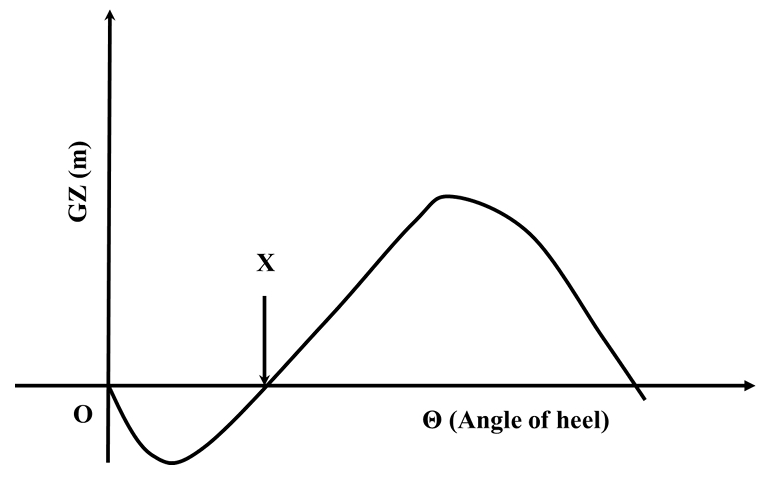
\includegraphics[width=0.4\columnwidth]{figs/fig-3.jpeg}
    \caption*{Fig-3:Curve for the question}
    \label{fig-3}
\end{figure}
\begin{enumerate}[leftmargin=2.5em, labelsep=0.5em, itemsep=0.5em]
      \item angle of loll 
      \item angle of vanishing stability 
      \item deck edge immersion angle 
      \item trim angle 
\end{enumerate}
\end{enumerate}

\begin{enumerate}[itemsep=1em]
\setcounter{enumi}{14}
\item Comparing a catamaran (with a separation between demi-hulls) and a mono-hull craft of the same displacement and water plane area, the initial metacentric radius of the catamaran will be 
\begin{enumerate}[leftmargin=2.5em, labelsep=0.5em, itemsep=0.5em]
     \item same as that of the mono-hull 
     \item one-half of the mono-hull 
     \item greater than that of the mono-hull 
     \item one-third of the mono-hull 
\end{enumerate}
\end{enumerate}
\newpage
\vspace*{0.25cm}

\begin{enumerate}[itemsep=1em]
\setcounter{enumi}{15}
\item The time series of rudder angle $(\delta)$ and heading angle $(\psi)$ during a ship's maneuver are shown in the following figure. Identify the maneuver and the associated parameters (p, q, r and s)
\begin{figure}[H]
    \centering
    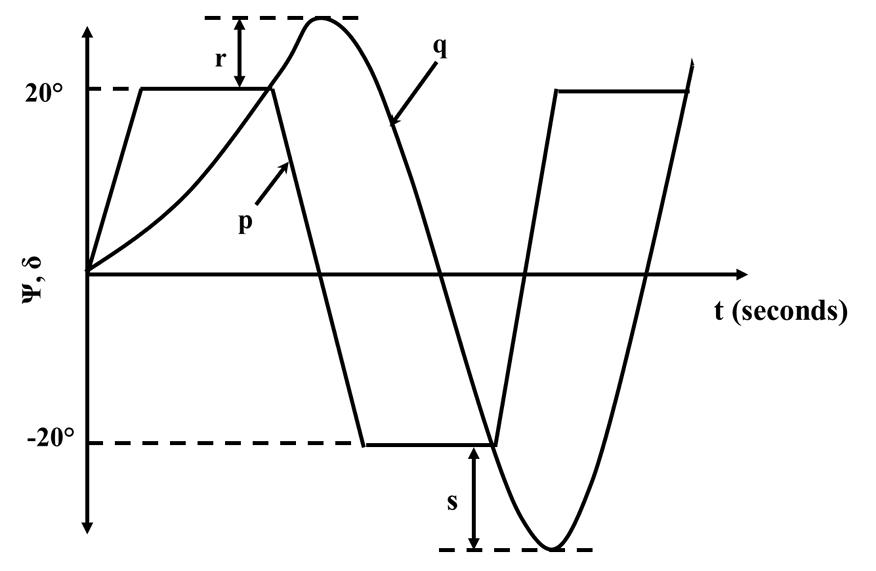
\includegraphics[width=0.4\columnwidth]{figs/fig-4.jpeg}
    \caption*{Fig-4:The time series of $\delta$ and $\psi$}
    \label{fig-4}
\end{figure}
\begin{enumerate}[leftmargin=2.5em, labelsep=0.5em, itemsep=0.5em]
    \item turning maneuver \\
p: heading angle, q: rudder angle, r: $1^{st}$ overshoot angle, s: $2^{nd}$ overshoot angle 
    \item spiral maneuver \\
p: heading angle, q: rudder angle, r: $1^{st}$ overshoot angle, s: $2^{nd}$ overshoot angle 
    \item zig-zag maneuver \\
p: rudder angle, q: heading angle, r: $1^{st}$ overshoot angle, s: $2^{nd}$ overshoot angle
    \item zig-zag maneuver \\
p: heading angle, q: rudder angle, r: $1^{st}$ overshoot angle, s: $2^{nd}$ overshoot angle
\end{enumerate}

\end{enumerate}

\begin{enumerate}[itemsep=1em]
\setcounter{enumi}{16}
\item A closed system undergoing a thermodynamic cycle consisting of two reversible isothermal and two reversible adiabatic processes is shown in the following figure. If $\delta Q$ is the infinitesimal heat transfer and T is the instantaneous 
temperature, then the value of the contour integral $\oint \frac{\delta Q}{T}$
\begin{figure}[H]
    \centering
    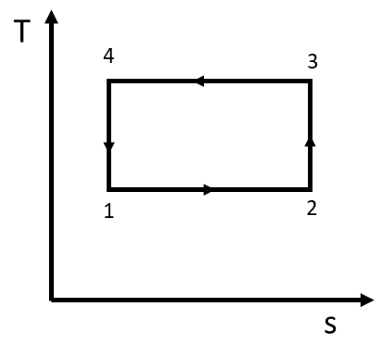
\includegraphics[width=0.4\columnwidth]{figs/fig-5.jpeg}
    \caption*{Fig-5:Thermodynamic cycle}
    \label{fig-5}
\end{figure}
\newpage
\vspace*{0.25cm}

\begin{enumerate}[leftmargin=2.5em, labelsep=0.5em, itemsep=0.5em]
      \item is positive 
      \item is negative 
      \item is zero 
      \item cannot be determined
\end{enumerate}

    
\end{enumerate}

\begin{enumerate}[itemsep=1em]
\setcounter{enumi}{17}
\item In a marine steam power cycle employing regeneration, the feed water heater for waste heat recovery is placed after the

\begin{multicols}{4}
\begin{enumerate}
      \item boiler
      \item turbine
      \item condenser
      \item pump
\end{enumerate}
\end{multicols}
\end{enumerate}

\begin{enumerate}[itemsep=1em]
\setcounter{enumi}{18}
\item From the following, choose the offshore platform that can be used ONLY for offshore drilling purpose. 

\begin{enumerate}[leftmargin=2.5em, labelsep=0.5em, itemsep=0.5em]
      \item Jacket platform 
      \item Jackup platform 
      \item Tension leg platform 
      \item SPAR
\end{enumerate}

\end{enumerate}

\begin{enumerate}[itemsep=1em]
\setcounter{enumi}{19}
\item Which method among the following is based on the strain energy principle? 
\begin{enumerate}[leftmargin=2.5em,labelsep=0.5em,itemsep=0.5em]
    \item Conjugate beam method 
    \item Castigliano's method
    \item Slope-deflection method 
    \item Moment distribution method 
\end{enumerate}
\end{enumerate}

\begin{enumerate}[itemsep=1em]
\setcounter{enumi}{20}
\item In dimensional analysis, according to Buckingham's $\pi$-theorem, if n is the total number of variables and m is the number of independent dimensions, then the maximum number of independent dimensionless $\pi$-groups will be 
\begin{multicols}{4}
\begin{enumerate}
       \item $m-n$
       \item $mn$
       \item $m+n$
       \item $n-m$
\end{enumerate}
\end{multicols}
\end{enumerate}

\begin{enumerate}[itemsep=1em]
\setcounter{enumi}{21}
\item  A submerged cylinder of diameter $1$ m is rotating clockwise at $100$ rpm, in a flow with a free stream velocity of $10$ m/s. Assuming ideal flow, the number of stagnation points on the cylinder is 
\begin{multicols}{4}
\begin{enumerate}
      \item $2$
      \item $3$
      \item $1$
      \item $0$
\end{enumerate}
\end{multicols}
\end{enumerate}

\newpage
\vspace*{0.25cm}

\begin{enumerate}[itemsep=1em]
\setcounter{enumi}{22}
\item The buoyancy curve variation of a ship floating in still water and in waves is shown in the following figure. The total area under each curve is the same. The cases 'X' and 'Y' correspond to 

\begin{figure}[H]
    \centering
    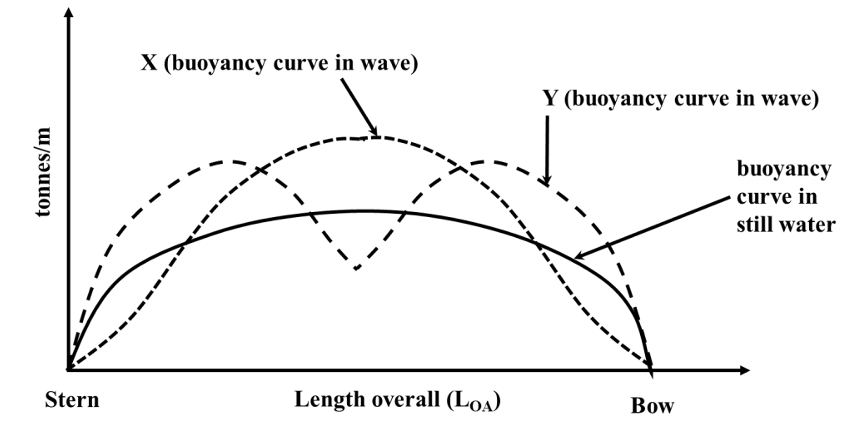
\includegraphics[width=0.6\columnwidth]{figs/fig-6.jpeg}
    \caption*{Fig-6:Buoyancy curve}
    \label{fig-6}
\end{figure}

\begin{enumerate}[leftmargin=2.5em, labelsep=0.5em, itemsep=0.5em]
    \item X: wave crest is amidships, Y: wave crest is amidships 
    \item X: wave trough is amidships, Y: wave trough is amidships 
    \item X: wave trough is amidships, Y: wave crest is amidships  
    \item X: wave crest is amidships, Y: wave trough is amidships
\end{enumerate}

\end{enumerate}

\begin{enumerate}[itemsep=1em]
\setcounter{enumi}{23}
\item Let $X$ be any random variable and $Y=-2X+3$.If $E[Y]=1$ and $E[Y^2]=9$, then which of the following are TRUE? 
\begin{multicols}{4}
\begin{enumerate}
    \item $E[X]=1$
    \item $E[X]=-2$
    \item $Var\,(X)=1$
    \item $Var\,(X)=2$
\end{enumerate}
\end{multicols}
\end{enumerate}

\begin{enumerate}[itemsep=1em]
\setcounter{enumi}{24}
\item Consider the contour integral $\oint \frac{dz}{z^4+z^3-2z^2}$  along the curve $|z| =3$ oriented in the counterclockwise direction. If $Res[f,z_0]$ denotes the residue of $f(z)$ at the point $z_0$,  then which of the following are TRUE? 

\begin{enumerate}[leftmargin=2.5em, labelsep=0.5em, itemsep=0.5em]
      \item $Res[f,0]=-1/4$
      \item $Res[f,1]=1/3$
      \item $Res[f,-2]=-1/12$
      \item $Res[f,2]=-1$
\end{enumerate}

\end{enumerate}

\newpage
\vspace*{0.25cm}

\begin{enumerate}[itemsep=1em]
\setcounter{enumi}{25}
\item A stationary ship has longitudinal symmetry. The surge, sway and heave motions are represented by indices $1-2-3$, respectively and roll, pitch and yaw motions are represented by indices $4-5-6$, respectively. Which of the following are TRUE 
about the added mass ($A_{ij}$)?
\begin{multicols}{4}
\begin{enumerate}
     \item $A_{35}=A_{53}$
     \item $A_{62}=A_{26}$
     \item $A_{46}=A_{64}$
     \item $A_{33}=A_{55}$
\end{enumerate}
\end{multicols}
\end{enumerate}

\begin{enumerate}[itemsep=1em]
\setcounter{enumi}{26}
\item The failure modes that may be observed in a riveted joint to fasten two plate members, subjected to shear load are  
\begin{enumerate}[leftmargin=2.5em, labelsep=0.5em, itemsep=0.5em]
        \item bending of the rivet 
        \item shearing of the rivet 
        \item tensile failure of a plate member 
        \item tensile failure of the rivet 
\end{enumerate}
\end{enumerate}

\begin{enumerate}[itemsep=1em]
\setcounter{enumi}{27}
\item A rectangular barge is freely floating in a drydock as shown in the following figure. For longitudinal strength analysis which of the following are TRUE?  
\begin{figure}[H]
    \centering
    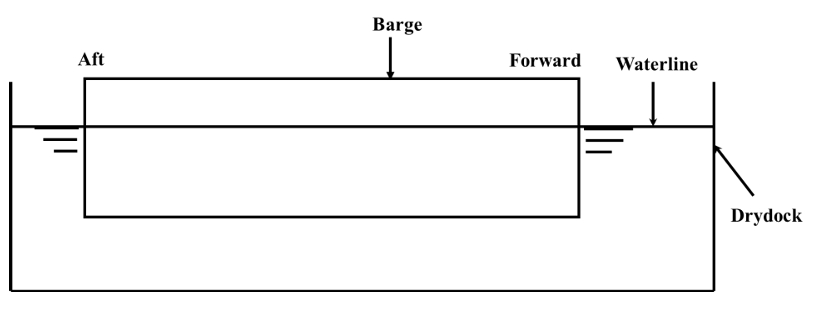
\includegraphics[width=0.6\columnwidth]{figs/fig-7.jpeg}
    \caption*{Fig-7:Rectangular barge}
    \label{fig-7}
\end{figure}
\begin{enumerate}[leftmargin=2.5em, labelsep=0.5em, itemsep=0.5em]
     \item The barge is considered as a free-free beam 
     \item At aft and forward ends: shear force = $0$, bending moment = $0$
     \item The barge is considered as a fixed-fixed beam 
     \item At aft and forward ends: shear force $\neq$ $0$, bending moment $\neq$ $0$
\end{enumerate}
\end{enumerate}

\begin{enumerate}[itemsep=1em]
\setcounter{enumi}{28}
\item A ship of length $180$ m has a displacement of $14400$ tonnes and is floating on an even keel in sea water of density $1025\; kg/m^3$. The trim changes by $0.18$ m when a weight of $120$ tonnes that is already onboard, is shifted $24$ m forward. The longitudinal metacentric height is \underline{\hspace{2cm}} m. 
\end{enumerate}

\newpage
\vspace*{0.25cm}
\begin{enumerate}[itemsep=1em]
\setcounter{enumi}{29}
\item A piezometer and a pitot tube measure the static and the total pressure of a fluid in a pipe flow respectively. The piezometer reads $100$ kPa and the pitot tube shows $200$ kPa. The density of the fluid is $1000\; kg/m^3$. The velocity of the flow is \underline{\hspace{1cm}} m/s (round off to one decimal place)  
\end{enumerate}

\begin{enumerate}[itemsep=1em]
\setcounter{enumi}{30}
\item A Carnot heat engine operates between two reservoirs of temperatures $900\;\degree C$ $(T_H)$ and $30\;\degree C$ $(T_L)$. If the heat transferred during one cycle to the engine from $T_H$ is $150$ kJ, then the energy rejected to $T_L$ is \underline{\hspace{1cm}} kJ (round off to the nearest integer) 
    
\end{enumerate}

\begin{enumerate}[itemsep=1em]
\setcounter{enumi}{31}
\item An oil tanker of breadth $20$ m and having a displacement of $24000$ tonnes in sea water (density of sea water = $1025 kg/m^3$) is carrying oil of relative density $0.8$ in $9$ longitudinally distributed tanks which are all half-filled. Each longitudinal tank is $12$ m long and $16$ m wide. The apparent change in vertical center of gravity, due to the presence of oil in the tanks is \underline{\hspace{1cm}} m (round off to one decimal place) 
\end{enumerate}

\begin{enumerate}[itemsep=1em]
\setcounter{enumi}{32}
\item For a regular sinusoidal wave propagating in deep water having wave height of $3.5$ m and wave period of $9$ s, the wave steepness is \underline{\hspace{1cm}} (round off to three decimal places)   
\end{enumerate}

\begin{enumerate}[itemsep=1em]
\setcounter{enumi}{33}
\item A solid cantilever shaft of diameter $0.1$ m and length $2$ m is subjected to a torque of $1$0 kN-m at the free end (shear modulus is $82$ GPa). The maximum induced shear stress is \underline{\hspace{1cm}} $N/mm^2$ (round off to the nearest integer). 
\end{enumerate}

\begin{enumerate}[itemsep=1em]
\setcounter{enumi}{34}
\item If a random variable $X$ has the probability density function 
\[
f(x) =
\begin{cases}
\frac{5}{32}x^4 & \text{if } 0 \le x \le 2, \\
0 & \text{otherwise } 
\end{cases}
\]
and if $Y=X^2$, then the expected value of $Y$ \underline{\hspace{2cm}} (round off to one decimal place) 
\end{enumerate}

\subsubsection{\underline{Q.36 \text{-} Q.65 Carry TWO mark Each}}
\begin{enumerate}[itemsep=1em]
\setcounter{enumi}{35}
\item The value of the surface integral $\iint\,(x^2dy\,dz +y^2 dz\,dx+z^2dx\,dy)$  over the surface of the cube given by $0 \le x \le 2$,$0 \le y \le 2$,$0 \le z \le 2$ is
\begin{multicols}{4}
\begin{enumerate}
    \item $12$
    \item $24$
    \item $36$
    \item $48$
\end{enumerate}
\end{multicols}
\end{enumerate}

\newpage
\vspace*{0.25cm}

\begin{enumerate}[itemsep=1em]
\setcounter{enumi}{36}
\item If the system of linear equations, $x-ay-z=0$, $ax-y-z=0$, $x+y-z=0$, has infinite number of solutions, then the possible values of $a$ are 
\begin{multicols}{4}
\begin{enumerate}
     \item $0,1$
     \item $-1,2$
     \item $-1,1$
     \item $0,-1$
\end{enumerate}
\end{multicols}
\end{enumerate}

\begin{enumerate}[itemsep=1em]
\setcounter{enumi}{37}
\item Two $30$ m long bilge keels of mass $40$ tonnes each, are fitted at the turn of the bilge on port and starboard sides of a ship. The cross section of the bilge keel is shown in the following figure. Assume density of water = $1000\;kg/m^3$. If the TPC (tonnes per centimeter) immersion of the ship is $50$, then the change in the mean draft is \underline{\hspace{1cm}} cm 
\begin{figure}[H]
    \centering
    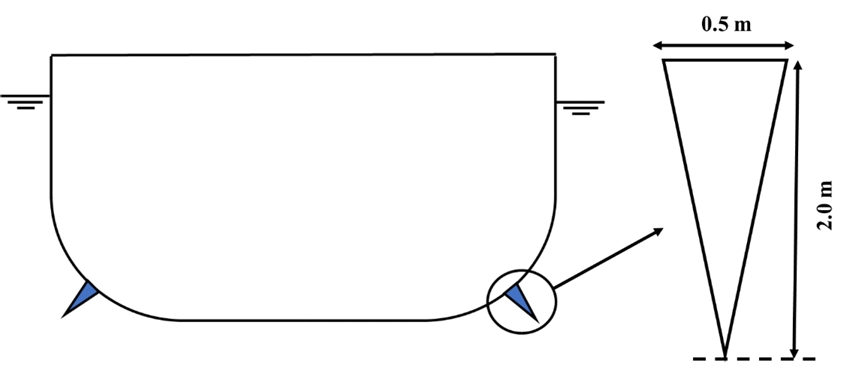
\includegraphics[width=0.6\columnwidth]{figs/fig-8.jpeg}
    \caption*{Fig-8:Cross-section of the bilge}
    \label{fig-8}
\end{figure}
\begin{multicols}{4}
\begin{enumerate}
    \item $1$
    \item $0.8$
    \item $0.6$
    \item $1.6$
\end{enumerate}
\end{multicols}
\end{enumerate}

\begin{enumerate}[itemsep=1em]
\setcounter{enumi}{38}
\item The layout of a Tension Leg Platform (TLP) is shown in the following figure.It consists of four interconnected pontoons at the bottom and four cylindrical columns, which support the working platform at the top. The density of sea water is $1025 \,kg/m^3$. Neglect the weight and buoyancy of the tethers. During operation, the maximum mass (in metric tonnes) of the entire structure must lie between
\begin{figure}[H]
    \centering
    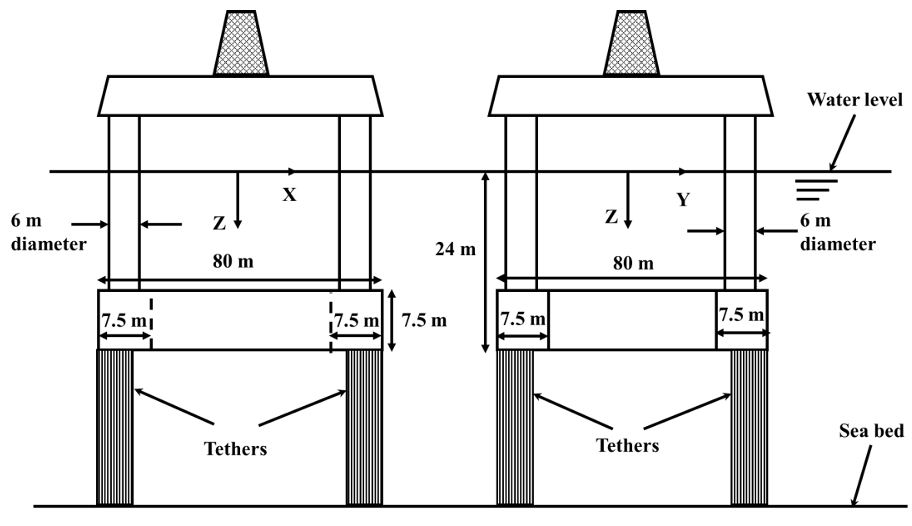
\includegraphics[width=0.6\columnwidth]{figs/fig-9.jpeg}
    \caption*{Fig-9:The layout of TLP}
    \label{fig-9}
\end{figure}
\newpage
\vspace*{0.25cm}
\begin{enumerate}[leftmargin=2.5em, labelsep=0.5em, itemsep=0.5em]
    \item $18630\;and\;18635$
    \item $28635\;and\;28640$ 
    \item $25655\;and\;25660$
    \item $24560\;and\;24565$
\end{enumerate}

\end{enumerate}

\begin{enumerate}[itemsep=1em]
\setcounter{enumi}{39}
\item The trajectory of a model ship during a pure sway PMM test is shown below.The steady forward speed, u is $2.0$ m/s. The maximum amplitude of sway motion,$y_{Max}$ is $0.5$ m and its period is $8$ s. The magnitude of maximum drift angle, in 
degrees (round off to the nearest integer), and the magnitude of maximum sway acceleration, in $m/s^2$ (round off to one decimal place), of the model respectively are
\begin{figure}[H]
    \centering
    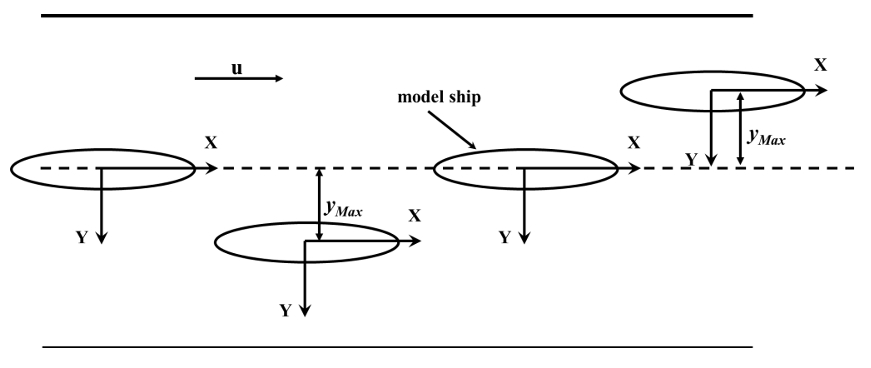
\includegraphics[width=0.6\columnwidth]{figs/fig-10.jpeg}
    \caption*{Fig-10:The trajectory of model ship}
    \label{fig-10}
\end{figure}

\begin{multicols}{4}
\begin{enumerate}
    \item $11\;and\;0.3$ 
    \item $13\;and\;0.5$
    \item $15\;and\;0.2$
    \item $9\;and\;0.1$
\end{enumerate}
\end{multicols}

\end{enumerate}

\begin{enumerate}[itemsep=1em]
\setcounter{enumi}{40}
\item ship of length 125 m has a design speed of $25$ knots ($1$ knot = $0.5144$ m/s). A $5.0$ m long geometrically similar model with wetted surface area of $4\,m^2$ has a coefficient of residuary resistance of $1.346 \times 10^{-3}$ at the corresponding speed. The ship's residuary resistance in kN (in sea water of density $1025\,kg/m^3$), and the model speed in knots (round off to the nearest integer) respectively are 
\begin{multicols}{4}
\begin{enumerate}
    \item $285\,and\,5$
    \item $17\;and\;5$
    \item $285\,and\,1$
    \item $17\;and\;1$
    
\end{enumerate}
\end{multicols}
\end{enumerate}

\newpage
\vspace*{0.25cm}

\begin{enumerate}[itemsep=1em]
\setcounter{enumi}{41}
\item A fully filled water tank $OABCD$ has a circular arc (AB) of radius $10$ m at the bottom as shown in the following figure. The height BC is 10 m. The length OA and CD are $5$ m and $15$ m, respectively. The density of the water is $\rho \ kg/m3$ and 
the acceleration due to gravity is $g \ m/s$. The magnitude of the resultant hydrostatic force per unit width acting on AB in N/m lies between 
\begin{figure}[H]
    \centering
    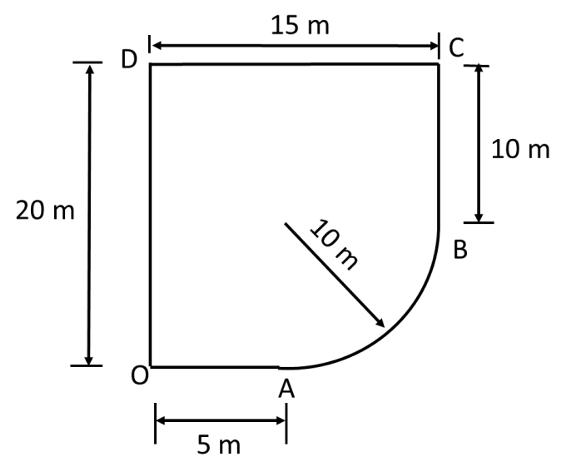
\includegraphics[width=0.6\columnwidth]{figs/fig-11.jpeg}
    \caption*{Fig-11: Water tank}
    \label{fig-11}
\end{figure}

\begin{enumerate}[leftmargin=2.5em, labelsep=0.5em, itemsep=0.5em]
     \item $190\rho g \ and \ 200\rho g$
     \item $210\rho g \ and \ 220\rho g$
     \item $230\rho g \ and \ 240\rho g$
     \item $250\rho g \ and \ 260\rho g$
\end{enumerate}


\end{enumerate}

\begin{enumerate}[itemsep=1em]
\setcounter{enumi}{42}
\item The velocity vector of a 2D flow field is given by $\vec{V} = 2y^2 \hat{i} + x^2 t$. The acceleration is  
\begin{enumerate}[leftmargin=2.5em, labelsep=0.5em, itemsep=0.5em]
     \item $4x^2ty \, \hat{i} + (x^2 + 4xy^2t) \hat{j}$
     \item $4x^2ty \, \hat{i} - (x^2 + 4xy^2t) \hat{j}$
     \item $4x^2ty \, \hat{i} + x^2 \hat{j}$
     \item $x^2 \hat{j}$

\end{enumerate}
   
\end{enumerate}

\newpage
\vspace*{0.25cm}

\begin{enumerate}[itemsep=1em]
\setcounter{enumi}{43}
\item 
Water is flowing with a free stream velocity of $0.25$ m/s around a submerged flat plate of $2$ m length (in the direction of flow) and $1$ m width. The local shear stress at a distance x from the leading edge of the plate is given by  
\[
\tau=\frac{0.332\rho u^2}{\sqrt{Re_x}}
\]
where $\rho= 1000 \ kg/m^3$ is the density of the water, $u$ is the free stream velocity and $Re_x$ is the Reynolds number at $x$. Assume that the flow is laminar, and the kinematic viscosity of water is $10^{-6}\  m^2/s$. The drag force (in Newton) acting on one side of the plate lies between  
\begin{multicols}{4}
\begin{enumerate}
    \item $0\ and\ 0.05$ 
    \item $0.05\ and\ 0.10$
    \item $0.10\ and\ 0.15$  
    \item $0.15\ and\ 0.20$  
\end{enumerate}
\end{multicols}
\end{enumerate}

\begin{enumerate}[itemsep=1em]
\setcounter{enumi}{44}
\item For a 2D ideal flow, let $\varphi$ be the velocity potential and $\psi$ be the stream function.Which one of the following is TRUE? 
\begin{enumerate}[leftmargin=2.5em, labelsep=0.5em, itemsep=0.5em]
    \item $\nabla^2 \varphi = 0 \;\; \text{and} \;\; |\nabla \psi|^2 = |\nabla \varphi|^2$
    \item $\nabla^2 \varphi = 0 \;\; \text{and} \;\; \nabla \psi \cdot \nabla \varphi \neq 0$
    \item $\nabla^2 \psi = 0 \;\; \text{and} \;\; |\nabla \psi|^2 \neq |\nabla \varphi|^2$
    \item $\nabla^2 \psi = 0 \;\; \text{and} \;\; \nabla \psi \times \nabla \varphi = 0$
\end{enumerate}
\end{enumerate}

\begin{enumerate}[itemsep=1em]
\setcounter{enumi}{45}
\item A long body with elliptical cross section is held perpendicular to a 2D uniform steady flow field of horizontal velocity $U_\infty$ as shown in the following figure. The 
heights of the control volume (bounded by the dashed lines) at the inlet and outlet are $2h$ and $4h$, respectively.  The profile of the horizontal velocity far downstream is given by 
$U(y)=\frac{U_\infty y}{2h}$.The density of the fluid is $\rho$. The magnitude of the drag force per unit length acting on the body is
\begin{figure}[H]
    \centering
    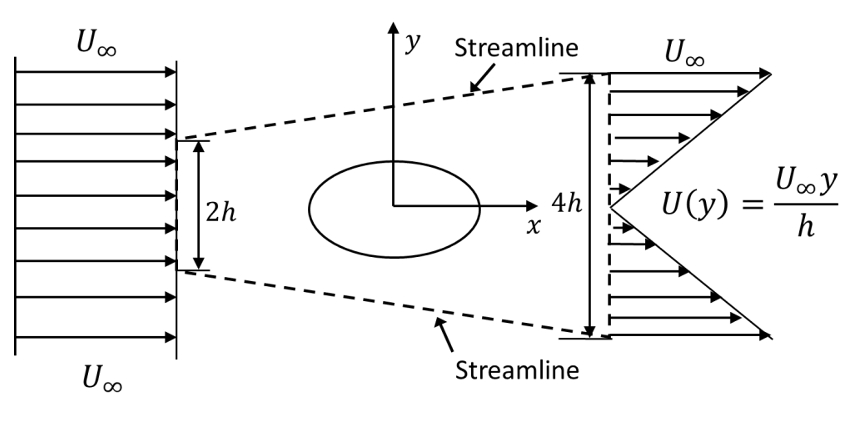
\includegraphics[width=0.5\columnwidth]{figs/fig-12.jpeg}
    \caption*{Fig-12}
    \label{fig-12}
\end{figure}
\begin{multicols}{4}
\begin{enumerate}
     \item $\frac{2\rho U_\infty^2 h}{3}$
     \item $\frac{\rho U_\infty^2 h}{3}$
     \item $\frac{\rho U_\infty^2 h}{2}$
     \item $\frac{2\sqrt{2}\rho U_\infty^2 h}{3}$
\end{enumerate}
\end{multicols}

\end{enumerate}

\newpage
\vspace*{0.25cm}

\begin{enumerate}[itemsep=1em]
\setcounter{enumi}{46}
\item A 'T' section is welded to the flat bottom shell plate of a ship as shown in the following figure (bottom shell longitudinal). The neutral axis of the ship's midship section is $14$ m above the bottom shell plate. The distance (X) of neutral 
axis of the 'T' section from the ship's neutral axis is \underline{\hspace{1cm}} m (round off to two decimal places) 
\begin{figure}[H]
    \centering
    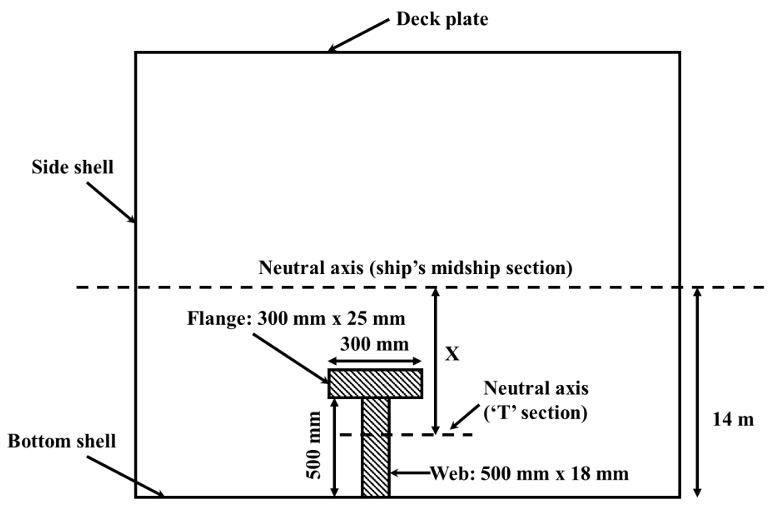
\includegraphics[width=0.5\columnwidth]{figs/fig-13.jpeg}
    \caption*{Fig-13:bottom shell longitudinal}
    \label{fig-13}
\end{figure}
\begin{multicols}{4}
\begin{enumerate}
    \item $12.63$
    \item $13.63$
    \item $15.24$
    \item $11.24$
\end{enumerate}
\end{multicols}
\end{enumerate}

\begin{enumerate}[itemsep=1em]
\setcounter{enumi}{47}
\item A vertical frictionless piston-cylinder arrangement contains air of mass $1$ kg. During a process, $50$ J of heat is transferred from outside to the system such that the piston is raised slowly by $0.1$ m from its initial equilibrium position. The mass of the piston is $1$ kg, and the diameter is $0.1$ m. Assume that $g = 9.81\ m/s^2$, and $P_{atm} = 100\ kPa$. The change in internal energy of the air in J (round off to two 
decimal places) lies between
\begin{figure}[H]
    \centering
    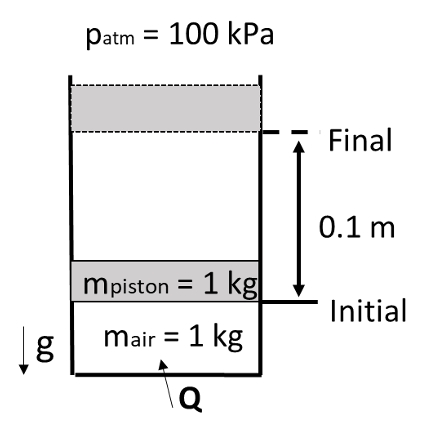
\includegraphics[width=0.4\columnwidth]{figs/fig-14.jpeg}
    \caption*{Fig-14:Piston-cyclinder arrangement}
    \label{fig-14}
\end{figure}
\newpage
\vspace*{0.25cm}
\begin{enumerate}[leftmargin=2.5em, labelsep=0.5em, itemsep=0.5em]
    \item $28.45 \ and \ 28.55$
    \item $-28.55 \ and \ -28.45$
    \item $-29.55 \ and \ -29.45 $
    \item $129.45 \ and \ 129.55 $
\end{enumerate}

\end{enumerate}

\begin{enumerate}[itemsep=1em]
\setcounter{enumi}{48}
\item An insulated nozzle has an inlet cross-sectional area of $314\ cm^2$. Air flows through the nozzle with an inlet temperature of $300$ K at a steady rate of $1.256\ m^3/s$. The velocity at the exit is greater than that at the inlet by $210\ m/s$.Assume a constant $C_p = 1.004$ kJ/kg-K. The temperature (in K) of air at the exit of the nozzle lies between   
\begin{multicols}{4}
\begin{enumerate}
    \item $330\ and \ 331 $
    \item $269\ and \ 270 $
    \item $320\ and \ 321 $
    \item $277\ and \ 278 $
    
\end{enumerate}
\end{multicols}
\end{enumerate}

\begin{enumerate}[itemsep=1em]
\setcounter{enumi}{49}
\item The heave natural frequencies of a Jacket structure, FPSO and a semi submersible are  $\omega_J$,$\omega_F$ and $\omega_S$ respectively. Each one of them has a pay load capacity of $10000$ tonnes.  Which of the following is TRUE?
\begin{multicols}{4}
\begin{enumerate}
    \item $\omega_J < \omega_F < \omega_S$
    \item $\omega_J > \omega_F > \omega_S$
    \item $\omega_J < \omega_S < \omega_F$
    \item $\omega_J > \omega_S > \omega_F$
\end{enumerate}
\end{multicols}
\end{enumerate}

\begin{enumerate}[itemsep=1em]
\setcounter{enumi}{50}
\item A simply supported beam with an overhang has experienced the bending moment as shown below. The corresponding concentrated load is
\begin{figure}[H]
    \centering
    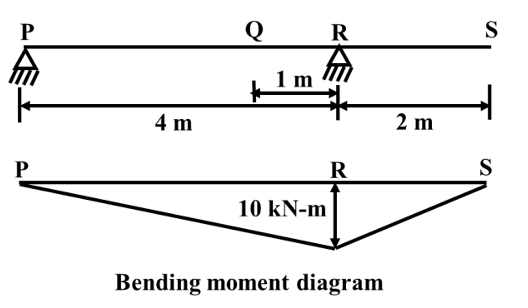
\includegraphics[width=0.4\columnwidth]{figs/fig-15.jpeg}
    \caption*{Fig-15}
    \label{fig-15}
\end{figure}
\begin{enumerate}[leftmargin=2.5em, labelsep=0.5em, itemsep=0.5em]
    \item $5$ kN at mid span of PR 
    \item $10$ kN at Q 
    \item $10$ kN at mid span of RS 
    \item $5$ kN at S 
\end{enumerate}
\end{enumerate}

\newpage
\vspace*{0.25cm}

\begin{enumerate}[itemsep=1em]
\setcounter{enumi}{51}
\item Let L=$\begin{myvec}{3&&-1&&-1&&-1 \\ -1&&2&&-1&&0 \\ -1&&-1&&3&&0 \\ -1&&0&&-1&&1}\end{myvec}$ . Which of the following are TRUE?
\begin{enumerate}[leftmargin=2.5em, labelsep=0.5em, itemsep=0.5em]
    \item The matrix L is row equivalent to $\begin{myvec}{0&&0&&0&&0 \\ -1&&2&&-1&&0 \\ -1&&-1&&3&&0 \\ -1&&0&&-1&&1}\end{myvec} $
    \item  The linear system $Lx=b$ has a solution for all $b$
    \item For $b \neq \begin{myvec}{1 \\ 1 \\ 1 \\ 1}\end{myvec}$ ,  the system $Lx=b$ has a solution 
    \item Rank of the matrix L is 3 
\end{enumerate}
\end{enumerate}

\begin{enumerate}[itemsep=1em]
\setcounter{enumi}{52}
\item For a given time varying load applied on a single degree of freedom system, the dynamic response amplitude is always less than the static response amplitude if 
\begin{enumerate}[leftmargin=2.5em, labelsep=0.5em, itemsep=0.5em]
    \item the applied loading frequency is greater than 1.5 times the natural frequency of the system
    \item the damping is greater than $70\%$ of critical damping 
    \item the damping is exactly $1/3^{rd}$ of critical damping 
    \item the applied loading frequency is less than the natural frequency of the system for an undamped system 
    
\end{enumerate}
\end{enumerate}

\begin{enumerate}[itemsep=1em]
\setcounter{enumi}{53}
\item The stress field, 
\begin{flushleft}
\[
\sigma_x = 4x^{3} + 3x^{2}y + 5xy^{2}
\]
\[
\sigma_y = -x^{3} + 6x^{2}y - 7xy^{2}
\]
\[
\tau_{xy} = -5x^{2}y - 3xy^{2}
\]
\end{flushleft}

would satisfy the strain compatibility condition if 
\begin{enumerate}[leftmargin=2.5em, labelsep=0.5em, itemsep=0.5em]
    \item both $\sigma_x$ and $\sigma_y$ are multiplied by $\frac{1}{2}$ 
    \item both $\sigma_x$ and $\sigma_y$ are multiplied by $2$
    \item $\tau_{xy}$ is multiplied by $\frac{1}{2}$
    \item $\tau_{xy}$ is multiplied by $2$
\end{enumerate}
\end{enumerate}

\newpage
\vspace*{0.25cm}

\begin{enumerate}[itemsep=1em]
\setcounter{enumi}{54}
\item If $y(x)$  is the solution of the differential equation  
\[
(1+x^2)y''-2xy'=0
\]
satisfying  $y(0)=0$ and  $y'(0)=3$, then  $y(1)$ equals \underline{\hspace{1cm}} 
\end{enumerate}

\begin{enumerate}[itemsep=1em]
\setcounter{enumi}{55}
\item For a ship of length $L = 100\ m$, the distance between the bow and stern pressure system is $0.942L$. Assume $g = 10 m/s^2$. The ship velocity corresponding to the prismatic hump of the wave making resistance curve is \underline{\hspace{3cm}} m/s (round off to one decimal place)  
\end{enumerate}

\begin{enumerate}[itemsep=1em]
\setcounter{enumi}{56}
\item A vessel of $100$ m length has a constant triangular cross-section with a depth of $12$ m and breadth of $15$ m as shown in following figure. The vessel has a vertical center of gravity (KG) = $6.675$ m. The minimum draft (d), at which the vessel 
will become stable is \underline{\hspace{1cm}} m (round off to one decimal place)
\begin{figure}[H]
    \centering
    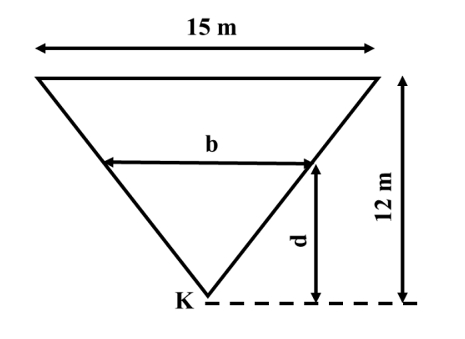
\includegraphics[width=0.4\columnwidth]{figs/fig-16.jpeg}
    \caption*{Fig-16:Triangular cross-section of the vessel}
    \label{fig-16}
\end{figure}

\end{enumerate}

\begin{enumerate}[itemsep=1em]
\setcounter{enumi}{57}
\item For a marine screw propeller, the open water characteristics at $J = 0.6$ are $KT  = 0.1336$ and $10KQ = 0.2010$. The open water propeller efficiency $\eta_o$, is 
\underline{\hspace{2cm}} (round off to two decimal places) 
\end{enumerate}

\begin{enumerate}[itemsep=1em]
\setcounter{enumi}{58}
\item Saturated liquid water (m = 1 kg) initially at $0.101$ MPa and $100\degree C$ is heated at constant pressure until the temperature increases to $500\degree C$. Assume a constant 
$C_p$ of steam = $1.9$ kJ/kg-K, and enthalpy of vaporization, $h_{fg}$ = $2257$ kJ/kg at $0.101$ MPa. The change in entropy of the water is \underline{\hspace{2cm}} kJ/K (round off to two decimal places) 
\end{enumerate}

\newpage
\vspace*{0.25cm}

\begin{enumerate}[itemsep=1em]
\setcounter{enumi}{59}
\item A simple vapor compression refrigeration cycle with ammonia as the working fluid operates between $30\degree C$ and $-10\degree C$ as shown in the following figure. The saturated liquid and vapor enthalpies at $30\degree C$ and $-10\degree C$ are provided in the table below. If the $COP$ of the cycle is $5.6$, the specific enthalpy at the inlet to the condenser is \underline{\hspace{2cm}} kJ/kg (round off to the nearest integer) 
\begin{table}[h]
\centering
\begin{tabular}{|c|c|c|}
\hline
Temperature ($^\circ$C) & $h_f$ (kJ/kg) & $h_g$ (kJ/kg) \\
\hline
30 & 320 & 1460 \\
\hline
-10  & 130 & 1420 \\
\hline
\end{tabular}
\end{table}

\begin{figure}[H]
    \centering
    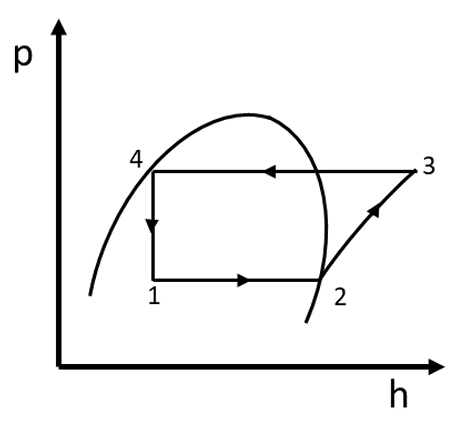
\includegraphics[width=0.4\columnwidth]{figs/fig-17.jpeg}
    \caption*{Fig-17: vapor compression refrigeration cycle}
    \label{fig-17}
\end{figure}
\end{enumerate}

\begin{enumerate}[itemsep=1em]
\setcounter{enumi}{60}
\item An air-standard diesel cycle, as shown in the following figure with a compression ratio of 16, has an initial pressure 0.9 bar and temperature 300 K. Assume $\gamma=1.4$ and $C_p = 1.004\ kJ/kg-K$. If the heat added during the constant pressure 
process is 900 kJ/kg, then the peak temperature during the cycle is \underline{\hspace{1cm}} K (round off to the nearest integer) 
\begin{figure}[H]
    \centering
    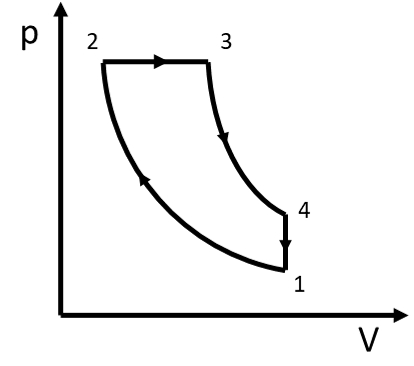
\includegraphics[width=0.4\columnwidth]{figs/fig-18.jpeg}
    \caption*{Fig-18: Air-standard diesel cycle}
    \label{fig-18}
\end{figure}
\end{enumerate}

\begin{enumerate}[itemsep=1em]
\setcounter{enumi}{61}
\item A tsunami that originated off the Indonesian coast has propagated towards the east-coast of India. It enters the continental shelf at 150 km away from the coast of Chennai. If the average water depth is 80 m from the coast to the continental shelf and 20 minutes is the tsunami period, the time taken by the tsunami to reach the coast of Chennai on entering the continental shelf is \underline{\hspace{1cm}} hours (round off to two decimal places) 
\end{enumerate}

\begin{enumerate}[itemsep=1em]
\setcounter{enumi}{62}
\item A buoy of virtual mass 30 kg oscillates in a fluid medium as a single degree of freedom system. If the total damping in the system is set as 188.5 N-s/m, such that the oscillation just ceases to occur, then the natural period of the system is 
\underline{\hspace{1cm}} s (round off to one decimal place) 
\end{enumerate}

\begin{enumerate}[itemsep=1em]
\setcounter{enumi}{63}
\item Consider a truss as shown in the following figure. The length of each member is 2 m. The area of cross section of each member is $100\ mm^2$ and Young's modulus is $2 \times 10^5\ N/mm^2$. The vertical deflection at C is \underline{\hspace{2cm}} mm (round off to one decimal place)
\begin{figure}[H]
    \centering
    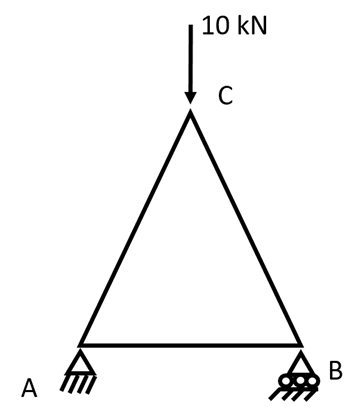
\includegraphics[width=0.4\columnwidth]{figs/fig-19.jpeg}
    \caption*{Fig-19:Truss}
    \label{fig-19}
\end{figure}
\end{enumerate}
\newpage
\vspace*{0.25cm}
\begin{enumerate}[itemsep=1em]
\setcounter{enumi}{64}
\item A marker buoy of mass 1500 kg floating in sea water of density $1025\ kg/m^3$, consists of a cylinder and cone as shown in the following figure. The buoy is suitably ballasted to make it stable in the floating condition. The buoy is subjected to an external periodic excitation force in Newton, $F_e(t)=2000\sin(1.25t)$.Ignore damping effects and assume $g = 9.81\ m/s^2$, added mass = 25\% of the mass of the buoy. The maximum heave response amplitude of the buoy is \underline{\hspace{1cm}} m (round off to one decimal place) 
\begin{figure}[H]
    \centering
    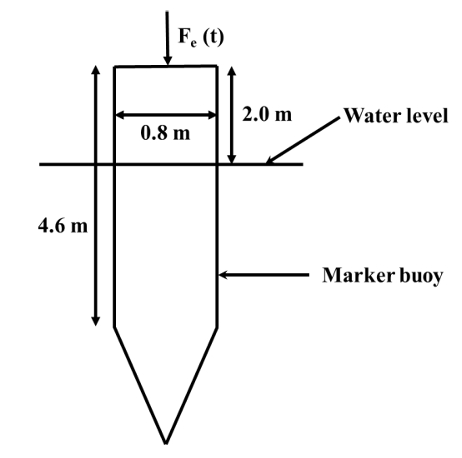
\includegraphics[width=0.4\columnwidth]{figs/fig-20.jpeg}
    \caption*{Fig-20:Marker buoy}
    \label{fig-20}
\end{figure}
\end{enumerate}


\end{document}
